\section{Restoring Solid Balance via ``Diamond-in-a-Diamond'' Convex Layers}
\label{sec:nested}

A striking mechanical contrast arises as soon as we compare the discrete vector cloud $P_S$ with its solid convex hull $\mathcal G_0(S):=\mathcal G(S)=\conv P_S$. By centring \eqref{eq:coords}, the $N=n^2$ discrete vectors always sum to $\sum_{i,j}\mathbf p_{ij}=\mathbf 0$. Yet for $829$ of the $880$ order-four magic squares, the uniform-density solid polyhedron $\mathcal G_0(S)$ has a non-zero centre of mass
\[
\mathbf c_0(S) := \mathbf c_{\mathrm{solid}}(\mathcal G_0(S)) = \frac{1}{\vol\mathcal G_0(S)}\iiint_{\mathcal G_0(S)}\mathbf x\,dV \ne \mathbf 0.
\]
Two geometric mechanisms drive this centroid drift:
\begin{enumerate}
\item \emph{Omission of non-vertex points:} The boundary $\partial\mathcal G_0(S)$ depends solely on the $V=|\vertset\mathcal G_0(S)|$ extreme points and ignores the positions of the $N-V$ interior and non-vertex boundary points $P_S^{(1)}=P_S\setminus\vertset\mathcal G_0(S)$.
\item \emph{Volumetric simplex weighting:} Even when $V=N=16$ (which occurs for $18$ of the $880$ order-four gems), a tetrahedral decomposition of $\mathcal G_0(S)$ from $O$ weights each simplex $\Delta_k$ by its volume $\vol(\Delta_k)$ rather than weighting the $16$ vertices equally.
\end{enumerate}

\subsection{Fifty-One Order-Four Gems Balance Naturally as Uniform Solids}

\begin{proposition}[Classification of the 51 naturally balanced order-four gems]
\label{prop:51-balanced}
Across the $880$ magic squares of order~$4$, the uniform solid $\mathcal G_0(S)$ has centre of mass $\mathbf c_0(S)=\mathbf 0$ for exactly $51$ squares:
\begin{enumerate}
\item The $48$ associative squares (Dudeney's Group~III), for which $z(-x,-y)=-z(x,y)$ implies $\mathcal G_0(S)=-\mathcal G_0(S)$, forcing $\mathbf c_0(S)=-\mathbf c_0(S)=\mathbf 0$ by central inversion.
\item Three non-associative squares in Dudeney's Group~VI: squares \#86, \#739, and \#756 (\Cref{tab:three-exceptions}).
\end{enumerate}
\end{proposition}

\begin{proof}
For every associative square $S$, $P_S=-P_S$ implies $\mathcal G_0(S)=-\mathcal G_0(S)$ and $\mathbf c_0(S)=\mathbf 0$. Each of the three Group~VI squares \#86, \#739, and \#756 is self-complementary via a reflection ($\overline S = hS$ or $\overline S = vS$), so $\mathcal G_0(S)$ is invariant under a $180^\circ$ half-turn $\iota_h\colon(x,y,z)\mapsto(x,-y,-z)$ or $\iota_v\colon(x,y,z)\mapsto(-x,y,-z)$ in $\R^3$ \cite[Prop.~4.3]{mathewson2026gems}. The half-turn forces two coordinates of $\mathbf c_0(S)$ to vanish identically ($c_{0,y}=c_{0,z}=0$ under $\iota_h$, or $c_{0,x}=c_{0,z}=0$ under $\iota_v$), and exact simplicial integration (\Cref{sec:appendix}) certifies that the single remaining rational axial moment vanishes exclusively on \#86, \#739, and \#756 among all $832$ non-associative squares.
\end{proof}

\begin{table}[htbp]
\centering
\caption{The three non-associative order-four magic squares whose uniform solid $\mathcal G_0(S)$ has exact centre of mass $\mathbf c_0(S)=\mathbf 0$, together with their inner core $\mathcal G_1(S)=\conv(P_S\setminus\vertset\mathcal G_0(S))$. All three squares lie in Dudeney's Group~VI and have $12$ outer vertices and $4$ inner points (spanning a planar parallelogram in \#86 and a 3D tetrahedron in \#739 and \#756) whose centroid $\mathbf c_1(S)$ is also $\mathbf 0$.}
\label{tab:three-exceptions}
\small
\setlength{\tabcolsep}{4.5pt}
\begin{tabular}{r c c c c c l}
\toprule
Square & Dudeney & $f(\mathcal G_0)$ & $\vol(\mathcal G_0)$ & $\operatorname{Iso}(\mathcal G_0)$ & $\dim/\vol(\mathcal G_1)$ & First row of standard form $S$\\
\midrule
\#86  & Group VI & $(12,28,18)$ & $209/3$ & $C_2$ ($\overline S=vS$) & $2\mathrm{D}$ ($0$) & $(1,7,14,12)$\\
\#739 & Group VI & $(12,26,16)$ & $287/3$ & $C_2$ ($\overline S=hS$) & $3\mathrm{D}$ ($5/3$) & $(4,14,3,13)$\\
\#756 & Group VI & $(12,24,14)$ & $84$    & $C_2$ ($\overline S=hS$) & $3\mathrm{D}$ ($4/3$) & $(5,2,15,12)$\\
\bottomrule
\end{tabular}
\end{table}

\subsection{Outer Hull Vertices and Inner Core Points Pull in Strictly Opposite Directions}

To restore exact physical balance around $O$ for the remaining $829$ gems without discarding the omitted grid points, we apply Chazelle's \emph{convex layer decomposition} (or onion peeling) \cite{chazelle1985convex} to $P_S$:
\begin{equation}
\label{eq:peeling}
P_S^{(0)} = P_S,\qquad
\mathcal G_k(S) = \conv P_S^{(k)},\qquad
P_S^{(k+1)} = P_S^{(k)} \setminus \vertset\mathcal G_k(S)\quad (k\ge0).
\end{equation}
We call $\mathcal G_0(S)$ the \emph{outer gem} and $\mathcal G_1(S)=\conv P_S^{(1)}\subset\mathcal G_0(S)$ the \emph{inner core gem}—geometrically, ``a diamond inside a diamond'' (\Cref{fig:nested-diamonds}(a,b)).

\begin{proposition}[Vertex-centroid opposition and order-four onion hierarchy]
\label{prop:opposition}
Let $S$ be any arrangement of order $n$ with $V=|\vertset\mathcal G_0(S)|<N$.
\begin{enumerate}
\item \emph{(Exact vertex-centroid opposition.)} The centroid $\overline{\mathbf p}_{\mathrm{outer}}=\frac1V\sum_{\mathbf p\in\vertset\mathcal G_0}\mathbf p$ of the outer vertices and the centroid $\overline{\mathbf p}_{\mathrm{inner}}=\frac{1}{N-V}\sum_{\mathbf p\in P_S^{(1)}}\mathbf p$ of the inner core points satisfy
\begin{equation}
\label{eq:opposition}
V\,\overline{\mathbf p}_{\mathrm{outer}} + (N-V)\,\overline{\mathbf p}_{\mathrm{inner}} = \mathbf 0.
\end{equation}
In particular, $\overline{\mathbf p}_{\mathrm{outer}}$ and $\overline{\mathbf p}_{\mathrm{inner}}$ are collinear with the origin $O$ and point in strictly opposite directions whenever $\overline{\mathbf p}_{\mathrm{outer}}\ne\mathbf 0$.
\item \emph{(Order-four layer census.)} Across the $880$ magic squares of order~$4$ (\Cref{fig:nested-diamonds}(c)):
\begin{itemize}
\item $18$ squares have $V=16$ ($P_S^{(1)}=\emptyset$, onion depth~$1$).
\item $842$ squares have onion depth~$2$, with $\dim\mathcal G_1(S)\in\{0,1,2,3\}$ distributed as $14$ singletons ($V=15$), $162$ collinear segments, $175$ planar polygons, and $491$ three-dimensional polyhedra $\mathcal G_1(S)$ all of whose points are vertices of $\mathcal G_1(S)$.
\item $20$ squares have onion depth~$3$ ($\mathcal G_0(S)\supset\mathcal G_1(S)\supset\mathcal G_2(S)$), comprising $16$ squares with dimension sequence $(3,3,0)$ (a 3D inner core gem enclosing a single innermost point) and $4$ squares with dimension sequence $(3,3,1)$ (a 3D inner core gem enclosing a 2-point segment).
\end{itemize}
In total, $491+16+4=511$ order-four magic squares possess a three-dimensional inner core gem $\mathcal G_1(S)$.
\end{enumerate}
\end{proposition}

\begin{proof}
Equation~\eqref{eq:opposition} follows immediately from $\sum_{\mathbf p\in P_S}\mathbf p=\mathbf 0$ and the partition $P_S=\vertset\mathcal G_0(S)\sqcup P_S^{(1)}$, and exact integer rank and convex-hull peeling across all $880$ squares yields the layer distribution in~(2).
\end{proof}

\begin{figure}[htbp]
\centering
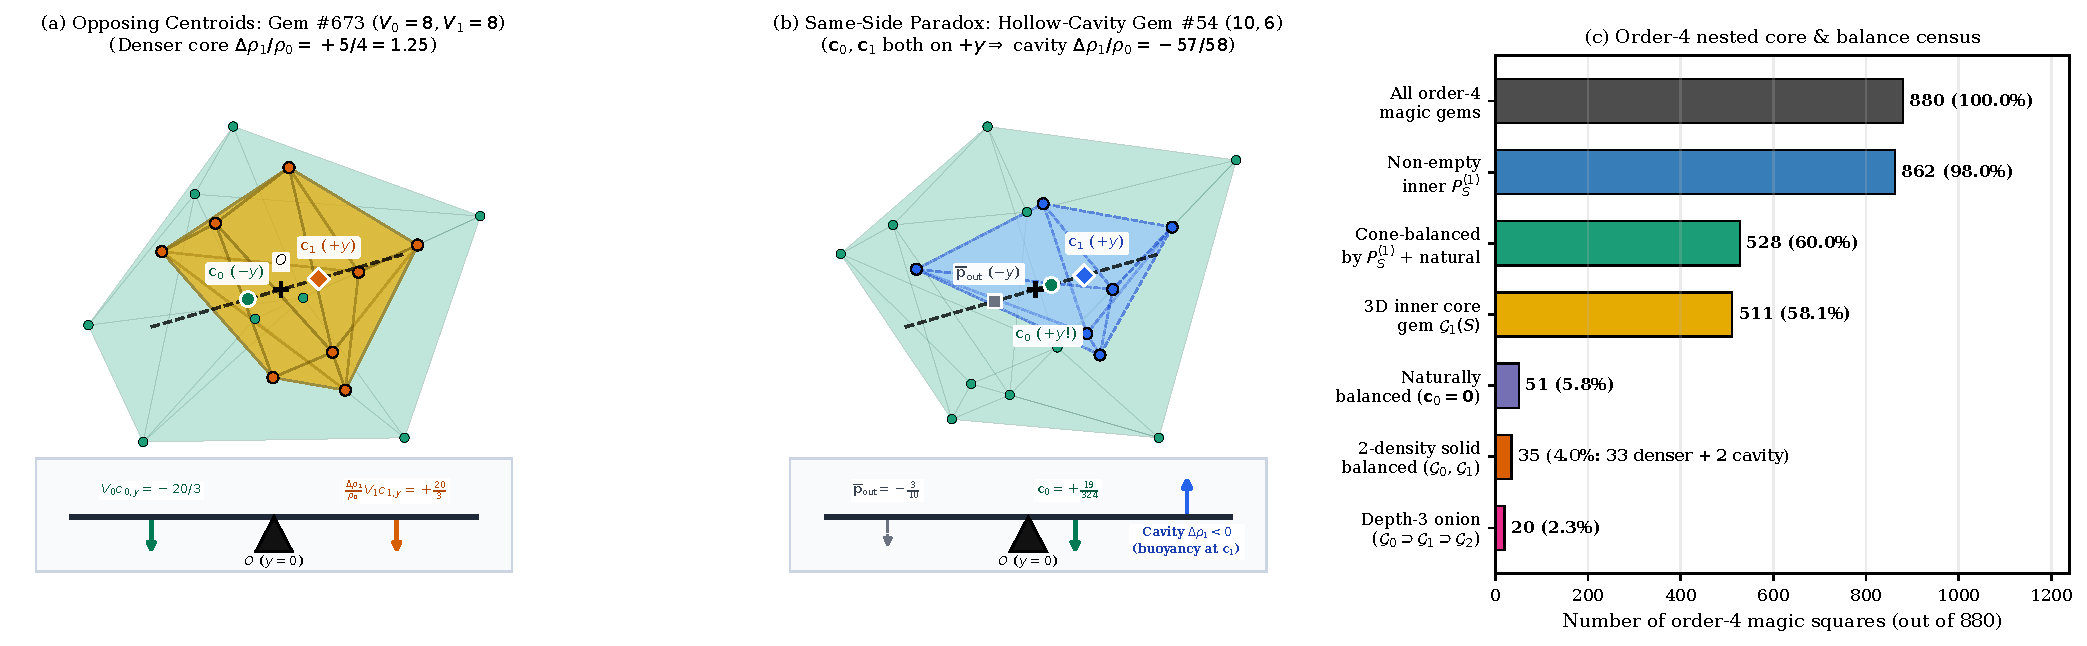
\includegraphics[width=\textwidth]{figures/fig_nested_diamonds.pdf}
\caption{Nested ``diamond-in-a-diamond'' convex layers $\mathcal G_0(S)\supset\mathcal G_1(S)$ and centre-of-mass restoration. (a)~Denser-core Gem \#673 ($(V_0,V_1)=(8,8)$, \Cref{fig:hero-squares}(e)) and (b)~hollow-cavity Gem \#54 ($(V_0,V_1)=(10,6)$, $1$-swap sibling of \#45 in \Cref{fig:hero-squares}(c)), showing the translucent outer hull $\mathcal G_0(S)$ enclosing the inner core gem $\mathcal G_1(S)$ alongside 2D fulcrum lever diagrams at bottom. On \#673, $\mathbf c_0=(0,0,-20/257)$ (green circle) and $\mathbf c_1=(0,0,+2/7)$ (gold diamond) lie on opposite sides of $O$, balancing via a heavier inner core ($\Delta\rho_1/\rho_0=+5/4$, $\rho_1/\rho_0=2.25$). On \#54, although the discrete outer vertices still pull to $-y$ ($\overline{\mathbf p}_{\mathrm{outer}}=(0,-3/10,0)$), volumetric simplex weighting pulls $\mathbf c_0=(0,+19/324,0)$ onto the $+y$ side alongside $\mathbf c_1=(0,+29/68,0)$, so subtracting a $98.3\%$ hollow core cavity ($\Delta\rho_1/\rho_0=-57/58$, $\rho_1/\rho_0=1/58$) restores balance at $O$. (c)~Breakdown of nested layer properties and balance mechanisms across all $880$ order-four magic squares.}
\label{fig:nested-diamonds}
\end{figure}

\subsection{Two-Density Core Inclusions and Inner-Core Weights Restore the Centre of Mass to the Origin}

Guided by \Cref{prop:opposition}, we establish three physical constructions that fabricate a continuous three-dimensional Magic Gem whose centre of mass lies at $O$.

\begin{theorem}[Composite ``diamond-in-a-diamond'' balancing]
\label{thm:diamond-balance}
Let $S$ be an order-four magic square.
\begin{enumerate}
\item \emph{(Two-density solid inclusion $(\mathcal G_0,\mathcal G_1)$.)} Suppose $\dim\mathcal G_1(S)=3$ ($511$ squares), and fabricate $\mathcal G_0(S)$ as a composite solid consisting of a baseline matrix of density $\rho_0>0$ throughout $\mathcal G_0(S)$ together with an inner core inclusion $\mathcal G_1(S)\subset\mathcal G_0(S)$ of excess density $\Delta\rho_1=\rho_1-\rho_0$. The composite centre of mass is
\[
\mathbf c_{\mathrm{comp}} = \frac{\rho_0\vol(\mathcal G_0)\,\mathbf c_0 + \Delta\rho_1\vol(\mathcal G_1)\,\mathbf c_1}{\rho_0\vol(\mathcal G_0) + \Delta\rho_1\vol(\mathcal G_1)}.
\]
Thus $\mathbf c_{\mathrm{comp}}=\mathbf 0$ for some $\Delta\rho_1\ne0$ if and only if $\mathbf c_0$ and $\mathbf c_1$ are non-zero and collinear ($\mathbf c_0\times\mathbf c_1=\mathbf 0$), with unique balancing density increment
\begin{equation}
\label{eq:density-ratio}
\frac{\Delta\rho_1}{\rho_0} = -\frac{\vol(\mathcal G_0)\,(\mathbf c_0\cdot\mathbf c_1)}{\vol(\mathcal G_1)\,\|\mathbf c_1\|_2^2}.
\end{equation}
The $511$ order-four gems with $\dim\mathcal G_1(S)=3$ partition into four exact classes:
\begin{itemize}
\item $207$ gems have $\mathbf c_1=\mathbf 0$ (comprising the $13$ associative gems with $\dim\mathcal G_1=3$ together with $194$ non-associative gems—including \#739 and \#756—whose four inner points form a tetrahedron with vertex sum $\mathbf 0$);
\item $254$ gems (outside Group~VI) have non-collinear solid centroids $\mathbf c_0\times\mathbf c_1\ne\mathbf 0$;
\item $33$ gems (all in Group~VI, where $C_2$ symmetry locks both $\mathbf c_0$ and $\mathbf c_1$ onto the symmetry axis) have strictly anti-parallel solid centroids ($\mathbf c_0\cdot\mathbf c_1<0$), balanced by a \emph{denser} inner core with rational excess density $\Delta\rho_1/\rho_0\in[5/4,\,191/6]$ (\Cref{tab:two-density} and \Cref{tab:all33}); for instance, on Gem \#673 (\Cref{fig:hero-squares}(e), \Cref{fig:nested-diamonds}(a)), eight extreme entries form a U-shaped outer cradle ($V_0=8$, $\overline{\mathbf p}_{\mathrm{outer}}=(0,-1/4,0)$) that swallows the eight intermediate T-core entries ($V_1=8$, $\overline{\mathbf p}_{\mathrm{inner}}=(0,+1/4,0)$), and loading $\mathcal G_1$ to $\Delta\rho_1/\rho_0=5/4$ balances the solid at $O$;
\item $17$ gems (also in Group~VI) have parallel solid centroids pointing in the \emph{same} direction ($\mathbf c_0\cdot\mathbf c_1>0$), because volumetric simplex weighting of $\mathcal G_0(S)\supset\mathcal G_1(S)$ pulls $\mathbf c_0$ to the same side of $O$ as $\mathbf c_1$ despite the opposite discrete vertex centroids of \eqref{eq:opposition}. Balancing these $17$ gems requires $\Delta\rho_1<0$, which is physically realizable with non-negative core density $\rho_1\in[0,\rho_0)$ ($|\Delta\rho_1|/\rho_0\le 1$) for two gems: square \#123 ($\Delta\rho_1/\rho_0=-3/17$, $\rho_1/\rho_0=14/17\approx0.824$, a lighter core) and square \#54 ($\Delta\rho_1/\rho_0=-57/58$, $\rho_1/\rho_0=1/58\approx0.017$, a nearly hollow core cavity, \Cref{fig:nested-diamonds}(b)). Notably, square \#54 is obtained from denser-core square \#45 ($\Delta\rho_1/\rho_0=+85/61$) by swapping a single complementary pair $(8,9)\leftrightarrow(15,2)$ in rows~$2$--$3$ (\Cref{fig:hero-squares}(c)): both have $(V_0,V_1)=(10,6)$, $\overline{\mathbf p}_{\mathrm{outer}}=(0,-3/10,0)$, and $\overline{\mathbf p}_{\mathrm{inner}}=(0,+1/2,0)$, yet inflating the $+y$ hull flares on \#54 pulls $\mathbf c_0$ across $O$ from $(0,-85/856,0)$ to $(0,+19/324,0)$ alongside $\mathbf c_1=(0,+29/68,0)$.
\end{itemize}
\item \emph{(Non-negative inner-core point weighting.)} If $\mathcal G_0(S)$ has uniform density $\rho_0$ and non-negative point masses $m_q\ge0$ are placed at the inner points $q\in P_S^{(1)}$, the composite solid balances at $O$ if and only if $-\mathbf c_0(S)\in\cone(P_S^{(1)})$. This cone condition holds for $477$ of the $829$ unbalanced gems; combined with the $51$ naturally balanced gems, $528$ of the $880$ order-four gems ($60.0\%$) achieve exact balance at $O$ via non-negative inner-core weights.
\item \emph{(Universal barycentric cell / bead-inlaid solid.)} For \emph{every} semi-magic square $S$ of any order $n$, partitioning $\mathcal G_0(S)$ into $N$ cells $C_{ij}$ of equal mass $M/N$ with cell centroids at $\mathbf p_{ij}$ (or embedding $N$ identical dense spherical beads of mass $m_{\mathrm{bead}}$ at $\mathbf p_{ij}$ in a light shell of density $\rho_0\to0$) yields $\mathbf c_{\mathrm{comp}}=\frac1N\sum_{i,j}\mathbf p_{ij}=\mathbf 0$ and restores the exact axisymmetric inertia tensor of \Cref{thm:rotor}.
\end{enumerate}
\end{theorem}

\begin{proof}
Part~(1) follows immediately from setting the first moment $\rho_0\vol(\mathcal G_0)\mathbf c_0+\Delta\rho_1\vol(\mathcal G_1)\mathbf c_1=\mathbf 0$ and evaluating the exact rational simplicial moments (\Cref{sec:appendix}) across all $511$ gems with $\dim\mathcal G_1(S)=3$. In Part~(2), existence of $m_q\ge0$ with $\rho_0\vol(\mathcal G_0)\mathbf c_0+\sum_{q\in P_S^{(1)}}m_q\mathbf p_q=\mathbf 0$ is equivalent to $-\mathbf c_0\in\cone(P_S^{(1)})$, certified by linear programming over the $829$ unbalanced gems. Part~(3) follows from $\sum_{i,j}\mathbf p_{ij}=\mathbf 0$ and \Cref{thm:rotor}.
\end{proof}

\begin{table}[htbp]
\centering
\caption{The eight order-four Magic Gems with the smallest balancing excess density ratios $\Delta\rho_1/\rho_0\in[5/4,40/19]\approx[1.25,2.11]$ in a two-density ``diamond-in-a-diamond'' solid inclusion $(\mathcal G_0(S),\mathcal G_1(S))$ (\Cref{thm:diamond-balance}(1)), all achievable with standard dual-material 3D printing. All $33$ denser-core gems belong to Dudeney's Group~VI, where $C_2$ symmetry forces even vertex counts $(V_0,V_1)$ and aligns $\mathbf c_0$ and $\mathbf c_1$ along the $x$- or $y$-axis. The complete list of $33$ gems is given in \Cref{tab:all33} and \texttt{anc/results\_paper\_c.json}.}
\label{tab:two-density}
\small
\setlength{\tabcolsep}{4.5pt}
\begin{tabular}{r r c c c c c c c}
\toprule
1-idx & 0-idx & $(V_0,V_1)$ & $\vol(\mathcal G_0)$ & $\vol(\mathcal G_1)$ & Axial $c_0$ & Axial $c_1$ & Exact $\Delta\rho_1/\rho_0$ & Decimal $\rho_1/\rho_0$\\
\midrule
\#673 & 672 & $(8,8)$  & $257/3$ & $56/3$ & $-20/257$  & $+2/7$    & $5/4$   & $2.250$\\
\#502 & 501 & $(10,6)$ & $271/3$ & $6$    & $+2/271$   & $-1/12$   & $4/3$   & $2.333$\\
\#45  & 44  & $(10,6)$ & $214/3$ & $6$    & $-85/856$  & $+61/72$  & $85/61$ & $2.393$\\
\#50  & 49  & $(10,6)$ & $254/3$ & $22/3$ & $-7/127$   & $+19/44$  & $28/19$ & $2.474$\\
\#307 & 306 & $(10,6)$ & $277/3$ & $22/3$ & $+23/1108$ & $-15/88$  & $23/15$ & $2.533$\\
\#49  & 48  & $(12,4)$ & $81$    & $2$    & $-2/81$    & $+1/2$    & $2$     & $3.000$\\
\#38  & 37  & $(10,6)$ & $263/3$ & $22/3$ & $+31/1052$ & $-15/88$  & $31/15$ & $3.067$\\
\#47  & 46  & $(10,6)$ & $247/3$ & $22/3$ & $-20/247$  & $+19/44$  & $40/19$ & $3.105$\\
\bottomrule
\end{tabular}
\end{table}

From a practical fabrication standpoint, the $33$ denser-core solids in \Cref{thm:diamond-balance}(1) split into two distinct regimes: the \emph{eight} gems in \Cref{tab:two-density} (\#673, \#502, \#45, \#50, \#307, \#49, \#38, and \#47) require a modest excess density ratio $\Delta\rho_1/\rho_0\in[5/4,\,40/19]\approx[1.25,\,2.11]$ (total core-to-shell density ratio $\rho_1/\rho_0\in[2.25,\,3.11]$), which is directly printable on a dual-extruder 3D printer using standard PLA ($\rho_0\approx1.24\,\mathrm{g/cm^3}$) around a tungsten- or bronze-filled composite filament core ($\rho_1\approx2.8\text{--}4.0\,\mathrm{g/cm^3}$), whereas the remaining $25$ gems in \Cref{tab:all33} have smaller inner-core volumes or shorter lever arms $\|\mathbf c_1\|_2$ and require $\Delta\rho_1/\rho_0\in[47/12,\,191/6]\approx[3.92,\,31.83]$. Overcoming this solid-density barrier—and extending exact balance to the $194$ gems whose tetrahedral core has $\mathbf c_{\mathrm{solid}}(\mathcal G_1)=\mathbf 0$—directly motivates the skeletal and thin-shell architectures of \Cref{subsec:wireframes-nets}: in a nested ball-and-rod wireframe $G(\mathcal G_0)\cup G(\mathcal G_1)$, linear rod mass density scales quadratically with diameter ($\rho_{\mathrm{lin}}\propto d^2$), compressing the required inner-to-outer rod diameter ratio by a square root ($d_1/d_0=\sqrt{\rho_{\mathrm{lin},1}/\rho_{\mathrm{lin},0}}$) and balancing $158$ Group~VI gems using a single homogeneous material.

\subsection{Ball-and-Rod Wireframes, Complete \texorpdfstring{$K_N$}{K\_N} Strut Networks, and Unfolded Papercraft Cutout Nets}
\label{subsec:wireframes-nets}

Beyond solid casting, the companion fabrication suite \cite{mathewson2025magicgemweb} realizes Magic Gems through three skeletal and thin-shell architectures (\Cref{fig:wireframes-nets}):
\begin{enumerate}
\item \emph{Outer and nested ball-and-rod wireframes $G(\mathcal G_0)\cup G(\mathcal G_1)$} (\texttt{magicGem\_v1.stl}), placing spherical or cubic nodes at the lifted points $\mathbf p_u(\lambda)$ and cylindrical rods along the $f_1(\mathcal G_0)$ edges of the outer hull $\mathcal G_0(S)$ and the $f_1(\mathcal G_1)$ edges of the inner core gem $\mathcal G_1(S)$ (\Cref{fig:wireframes-nets}(a));
\item \emph{Fully interconnected complete strut networks $K_N\bigl(P_S(\lambda)\bigr)$} (\texttt{magicGem\_v2.stl}), connecting all $\binom{N}{2}$ pairs of lifted points $\mathbf p_u(\lambda),\mathbf p_v(\lambda)$ ($120$ rods at $n=4$: $f_1(\mathcal G_0)$ outer boundary edges plus $120-f_1(\mathcal G_0)$ internal cross-struts running through the interior of the hull, \Cref{fig:wireframes-nets}(b)); and
\item \emph{Unfolded 2D papercraft cutout nets with trapezoidal glue tabs}, unfolding the boundary surface $\partial\mathcal G_\lambda(S)$ into a flat printable net along a breadth-first spanning tree of the dual facet graph $G^*(\mathcal G)$ (\Cref{fig:wireframes-nets}(c)).
\end{enumerate}

\begin{theorem}[Universal covariance of the complete $K_N$ strut network versus length-weighted and nested wireframes]
\label{thm:complete-network}
Let $S$ be an arrangement of $\{1,\dots,N\}$, $N=n^2$ ($n\ge2$), with lifted point cloud $P_S(\lambda)=\{\mathbf p_1(\lambda),\dots,\mathbf p_N(\lambda)\}\subset\R^3$ satisfying $\sum_{u=1}^N\mathbf p_u(\lambda)=\mathbf 0$ and empirical covariance matrix $\Sigma(\lambda)=\frac1N\sum_{u=1}^N\mathbf p_u(\lambda)\mathbf p_u(\lambda)^{\top}$. In the one-dimensional slender-rod (line-skeleton) limit $d/L_{uv}\to 0^+$, where each rod is concentrated along its centreline segment:
\begin{enumerate}
\item \emph{(Equal-mass-per-edge complete network $K_N$.)} Suppose each of the $\binom{N}{2}$ slender rods connecting $\mathbf p_u(\lambda)$ and $\mathbf p_v(\lambda)$ ($1\le u<v\le N$) carries equal mass $m_{\mathrm{edge}}=M_{\mathrm{rods}}/\binom{N}{2}$ (together with optional equal node masses $m_{\mathrm{node}}=M_{\mathrm{nodes}}/N$ at the $N$ vertices, where $M_{\mathrm{nodes}}=\theta M$ and $M_{\mathrm{rods}}=(1-\theta)M$ for $\theta\in[0,1]$). Because $K_N$ is $(N-1)$-regular, the centre of mass of $K_N\bigl(P_S(\lambda)\bigr)$ lies at the origin $O$ for \emph{every} arrangement $S$:
\begin{equation}
\label{eq:kN-com}
\mathbf c\bigl(K_N(\lambda)\bigr) = \frac{1}{\binom{N}{2}}\sum_{1\le u<v\le N}\frac{\mathbf p_u(\lambda)+\mathbf p_v(\lambda)}{2} = \frac{1}{N}\sum_{u=1}^N\mathbf p_u(\lambda) = \mathbf 0.
\end{equation}
Furthermore, the continuous second-moment covariance matrix of the $\binom{N}{2}$ equal-mass slender rods is an exact universal scalar multiple of the discrete covariance matrix $\Sigma(\lambda)$:
\begin{equation}
\label{eq:kN-cov}
\Sigma_{\mathrm{rods}}^{(=\text{mass})}\bigl(K_N(\lambda)\bigr)
= \frac{2N-3}{3(N-1)}\,\Sigma(\lambda)
\qquad\Bigl(=\frac{5}{8}\,\Sigma(\lambda)\text{ at }n=3,\quad \frac{29}{45}\,\Sigma(\lambda)\text{ at }n=4\Bigr).
\end{equation}
Consequently, for \emph{every} semi-magic square $S$ of order $n$ and every node-mass fraction $\theta\in[0,1]$, the composite complete network $K_N\bigl(P_S(\lambda)\bigr)$ has covariance $\bigl(\theta+(1-\theta)\frac{2N-3}{3(N-1)}\bigr)\Sigma(\lambda)$ and therefore shares the \emph{exact same axisymmetric inertia ratio $I_\perp(\lambda)/I_{zz}=\frac12\bigl(1+\lambda^2(n^2+1)\bigr)$, the exact same spherical-top scale $\lambda_{\mathrm{iso}}=(n^2+1)^{-1/2}$, and the exact same integer polhode ratio $(n^2+2)/2=9$ at $\lambda=1$} as the discrete point cloud in \Cref{thm:rotor}.
\item \emph{(Length-weighted strut networks $\rho_{\mathrm{lin}}=\mathrm{const}$.)} When a subgraph $G=(V_G,E_G)$ is fabricated from slender rods of uniform cross-sectional diameter $d$ and linear mass density $\rho_{\mathrm{lin}}=\frac\pi4 d^2\rho_{\mathrm{mat}}$, each rod $(u,v)\in E_G$ has mass proportional to its Euclidean length $L_{uv}(\lambda)=\|\mathbf p_u(\lambda)-\mathbf p_v(\lambda)\|_2$, total rod length $L(G;\lambda)=\sum_{(u,v)\in E_G}L_{uv}(\lambda)$, and length-weighted centroid
\[
\mathbf c_{\mathrm{len}}(G;\lambda) = \frac{1}{2L(G;\lambda)}\sum_{u\in V_G}\Biggl(\sum_{v:\,(u,v)\in E_G}L_{uv}(\lambda)\Biggr)\mathbf p_u(\lambda).
\]
Across all $880$ order-four magic squares (\Cref{fig:wireframes-nets}(d)):
\begin{itemize}
\item Both the $120$-rod complete network $K_{16}$ and the outer hull wireframe $G(\mathcal G_0)$ have $\mathbf c_{\mathrm{len}}=\mathbf 0$ if and only if $S$ is one of the $48$ centrally symmetric associative squares ($5.5\%$).
\item Passing from the outer hull wireframe $G(\mathcal G_0)$ (mean total rod length $\overline L=143.30$ at $\lambda=1$ and $60.00$ at $\lambda=0.20$) to the complete $120$-rod network $K_{16}$ ($\overline L=756.14$ at $\lambda=1$ and $305.34$ at $\lambda=0.20$) reduces the mean centroid drift $\|\mathbf c_{\mathrm{len}}\|_2$ by $2.7\times$ at $\lambda=1$ (from $0.1940$ to $0.0717$) and by $3.6\times$ at $\lambda=0.20$ (from $0.0879$ to $0.0247$, versus $0.0888$ for the uniform solid), while tightening the mean transverse inertia splitting $(I_3-I_2)/I_2$ to $0.0051$ at $\lambda=1$.
\end{itemize}
\item \emph{(Composite balance of nested wireframes $G(\mathcal G_0)\cup G(\mathcal G_1)$ via rod diameter tuning.)} For the $848$ order-four gems with $\dim\mathcal G_1(S)\ge1$, fabricating the outer edges $E(\mathcal G_0)$ with rod diameter $d_0$ and the disjoint inner core edges $E(\mathcal G_1)$ with rod diameter $d_1$ yields $\mathbf c_{\mathrm{wire}}(\mathcal G_0\cup\mathcal G_1)=\mathbf 0$ whenever $\mathbf c_{\mathrm{wire}}(\mathcal G_0)$ and $\mathbf c_{\mathrm{wire}}(\mathcal G_1)$ are strictly anti-parallel, at the unique rod diameter ratio
\begin{equation}
\label{eq:rod-diam-ratio}
\frac{d_1}{d_0} = \sqrt{\frac{\rho_{\mathrm{lin},1}}{\rho_{\mathrm{lin},0}}}
= \sqrt{-\frac{L\bigl(G(\mathcal G_0)\bigr)\,\bigl(\mathbf c_{\mathrm{wire}}(\mathcal G_0)\cdot\mathbf c_{\mathrm{wire}}(\mathcal G_1)\bigr)}{L\bigl(G(\mathcal G_1)\bigr)\,\|\mathbf c_{\mathrm{wire}}(\mathcal G_1)\|_2^2}}.
\end{equation}
Because $E(\mathcal G_0)\cap E(\mathcal G_1)=\emptyset$, any ratio $d_1/d_0>0$ is physically realizable without cavity constraints. Consequently, exact composite wireframe balance holds for $158$ Group~VI gems at $\lambda=1$ ($81$ with $\dim\mathcal G_1=3$, $37$ with $\dim\mathcal G_1=2$, $40$ with $\dim\mathcal G_1=1$; e.g., Gem \#673 at $d_1/d_0=0.7932$ and Gem \#45 at $d_1/d_0=0.7945$) and for $164$ Group~VI gems at $\lambda=0.20$ ($83$ with $\dim\mathcal G_1=3$; e.g., Gem \#673 at $d_1/d_0=0.4932$ and Gem \#45 at $d_1/d_0=0.7694$).
\end{enumerate}
\end{theorem}

\begin{proof}
(1) Integrating $\mathbf x(t)=(1-t)\mathbf p_u+t\mathbf p_v$ over $t\in[0,1]$ gives the rod midpoint $\frac12(\mathbf p_u+\mathbf p_v)$ and second-moment matrix
\[
M_2(u,v) = \int_0^1 \mathbf x(t)\mathbf x(t)^{\top}\,dt = \frac{1}{3}\bigl(\mathbf p_u\mathbf p_u^{\top} + \mathbf p_v\mathbf p_v^{\top}\bigr) + \frac{1}{6}\bigl(\mathbf p_u\mathbf p_v^{\top} + \mathbf p_v\mathbf p_u^{\top}\bigr).
\]
In $K_N$, each vertex $u$ belongs to $N-1$ edges, proving \eqref{eq:kN-com} and giving $\sum_{u<v}(\mathbf p_u\mathbf p_u^{\top}+\mathbf p_v\mathbf p_v^{\top})=(N-1)\sum_{u=1}^N\mathbf p_u\mathbf p_u^{\top}=N(N-1)\Sigma(\lambda)$. Similarly, expanding $\mathbf 0=\bigl(\sum_u\mathbf p_u\bigr)\bigl(\sum_v\mathbf p_v\bigr)^{\top}$ yields $\sum_{u<v}(\mathbf p_u\mathbf p_v^{\top}+\mathbf p_v\mathbf p_u^{\top})=-\sum_{u=1}^N\mathbf p_u\mathbf p_u^{\top}=-N\Sigma(\lambda)$. Dividing by $\binom{N}{2}=\frac12N(N-1)$ gives
\[
\Sigma_{\mathrm{rods}}^{(=\text{mass})}\bigl(K_N(\lambda)\bigr)
= \frac{2}{N(N-1)}\left(\frac{N-1}{3} - \frac{1}{6}\right)N\Sigma(\lambda)
= \frac{2N-3}{3(N-1)}\,\Sigma(\lambda),
\]
establishing \eqref{eq:kN-cov}. Parts~(2) and~(3) follow by evaluating $L(G;\lambda)$, $\mathbf c_{\mathrm{len}}(G;\lambda)$, and \eqref{eq:rod-diam-ratio} across all $880$ squares (\Cref{sec:appendix}).
\end{proof}

\begin{proposition}[Papercraft cutout nets, topological glue-tab invariant, and thin-shell balance]
\label{prop:papercraft-net}
Let $\mathcal G_\lambda(S)$ be any three-dimensional Magic Gem with $f$-vector $(f_0,f_1,f_2)$.
\begin{enumerate}
\item \emph{(Universal glue-tab invariant $N_{\mathrm{tabs}}=f_0-1$ and non-overlapping order-four nets.)} Unfolding $\partial\mathcal G_\lambda(S)$ into a connected planar cutout net along any spanning tree $T^*$ of the dual facet graph $G^*(\mathcal G)$ \cite{durer1525underweysung,shephard1975convex,demaine2007geometric,ghomi2014durer} partitions the $f_1$ polyhedral edges into $|E_{\mathrm{fold}}|=f_2-1$ interior fold lines (dashed creases in \Cref{fig:wireframes-nets}(c)) and $N_{\mathrm{tabs}}=f_1-(f_2-1)$ cut edges, each opened into a pair of exterior boundary segments joined by one trapezoidal glue tab (labelled in matching pairs \texttt{a}--\texttt{k} in \Cref{fig:wireframes-nets}(c)). Because $\partial\mathcal G_\lambda(S)\cong S^2$ is a genus-$0$ planar surface, the cut edges $E\setminus E(T^*)$ form a complementary spanning tree $T$ of the primal $1$-skeleton $G(\mathcal G_\lambda)$ on the $f_0$ hull vertices (equivalently, the cycle rank $\beta_1(G^*)=f_1-f_2+1$ of the dual graph equals $f_0-1$ by Euler's formula $f_0-f_1+f_2=2$), so the number of glue tabs depends \emph{solely on the hull vertex count $f_0$}:
\begin{equation}
\label{eq:glue-tabs}
N_{\mathrm{tabs}} = f_1 - (f_2 - 1) = |E(T)| = f_0 - 1,
\end{equation}
and the net perimeter consists of $2(f_0-1)$ cut boundary segments. Moreover, \eqref{eq:glue-tabs} is strictly invariant under triangulating non-triangular facets into $F_\Delta=2f_0-4$ triangles and $E_\Delta=3f_0-6$ edges, since $E_\Delta-(F_\Delta-1)=(3f_0-6)-(2f_0-5)=f_0-1$. Across the $880$ order-four Magic Gems, $N_{\mathrm{tabs}}=f_0-1$ takes every integer value in $\{7,\dots,15\}$ (distributed as $7$ gems with $7$ tabs, $10$ with $8$, $103$ with $9$, $80$ with $10$, $380$ with $11$ including D\"urer's gem \#175, $106$ with $12$, $162$ with $13$, $14$ with $14$, and $18$ with $15$ tabs). Under the deterministic breadth-first dual spanning tree $T^*$ rooted at the largest-area facet $F_0$ (marked $\bigstar F_0$ in \Cref{fig:wireframes-nets}(c), visiting adjacent facets in canonical index order), \emph{all $880$ order-four Magic Gems ($100\%$) unfold into strictly non-overlapping 2D planar nets} at both $\lambda=1$ and $\lambda=0.20$.
\item \emph{(Hollow thin-shell mechanics $\partial\mathcal G_\lambda(S)$ and nested shell balance.)} In the idealized mathematical shell model $\partial\mathcal G_\lambda(S)$ of uniform areal mass density $\sigma_0>0$ (with massless glue tabs, or butt-jointed laser-cut facets), the surface area is $\operatorname{area}(\partial\mathcal G_\lambda)\in[116.53,148.62]$ (mean $135.13$) at $\lambda=1$ and $[31.26,40.02]$ (mean $36.38$) at $\lambda=0.20$, with area-weighted centroid $\mathbf c_{\mathrm{shell}}(\mathcal G_0)=\frac{1}{\operatorname{area}(\partial\mathcal G_0)}\sum_F A_F\mathbf c(F)$ vanishing on all $48$ associative squares and having mean drift $0.1357$ at $\lambda=1$ ($0.0907$ at $\lambda=0.20$). Enclosing a nested inner shell $\partial\mathcal G_1(S)$ ($\dim\mathcal G_1=3$) of areal density $\sigma_1$ restores exact composite balance $\mathbf c_{\mathrm{shell}}(\partial\mathcal G_0\cup\partial\mathcal G_1)=\mathbf 0$ for $80$ Group~VI gems at $\lambda=1$ and $87$ Group~VI gems at $\lambda=0.20$ (including Gem \#673 at $\sigma_1/\sigma_0=0.9110$ for $\lambda=1$ and $0.6826$ for $\lambda=0.20$, and Gem \#45 at $\sigma_1/\sigma_0=0.0849$ for $\lambda=1$ and $0.2003$ for $\lambda=0.20$).
\end{enumerate}
\end{proposition}

\begin{proof}
By planar graph duality on $\partial\mathcal G_\lambda(S)\cong S^2$, the complement of a dual spanning tree $T^*\subset G^*(\mathcal G_\lambda)$ ($|E(T^*)|=f_2-1$) is a primal spanning tree $T\subset G(\mathcal G_\lambda)$ on the $f_0$ vertices, giving $N_{\mathrm{tabs}}=|E(T)|=f_0-1$ directly (and matching $f_1-(f_2-1)=f_0-1$ by Euler's formula). Whether every convex polyhedron admits a non-overlapping edge unfolding remains open in general (D\"urer's conjecture \cite{durer1525underweysung,shephard1975convex,demaine2007geometric,ghomi2014durer}); for the $880$ order-four Magic Gems at $\lambda=1$ and $\lambda=0.20$, exact 2D polygon intersection testing of the breadth-first dual spanning-tree unfolding and exact triangular surface moments certify non-overlap and the stated shell censuses across all $880$ gems (\Cref{sec:appendix}).
\end{proof}

\begin{remark}[Finite-diameter cylinders, hub intersections, and core suspension]
\label{rem:finite-diameter}
In a physical 3D print of finite rod diameter $d>0$, each right circular cylinder of length $L_{uv}$ and unit direction $\hat{\mathbf e}_{uv}=(\mathbf p_v-\mathbf p_u)/L_{uv}$ has midpoint centroid $\frac12(\mathbf p_u+\mathbf p_v)$ (leaving \eqref{eq:kN-com} unchanged) and adds the transverse radial inertia correction $m_{uv}\frac{d^2}{16}(I_3+\hat{\mathbf e}_{uv}\hat{\mathbf e}_{uv}^{\top})$ to its slender-rod inertia tensor, while boolean union at the $16$ degree-$15$ vertex hubs and interior strut crossings subtracts $O(d^3)$ cap-overlap volumes. To suspend the disjoint inner core wireframe $G(\mathcal G_1)$ inside $G(\mathcal G_0)$ on a Group~VI gem, one connects them by either lightweight tension filaments or $C_2$-symmetric pairs of equal-length struts whose midpoint centroid lies at $O$, leaving the balancing diameter ratio $d_1/d_0$ in \eqref{eq:rod-diam-ratio} invariant. Finally, the jump from $35$ two-density balanced solids (\Cref{thm:diamond-balance}(1)) to $158$ balanced nested wireframes at $\lambda=1$ arises because $194$ non-associative gems have a $4$-vertex tetrahedral core $\mathcal G_1(S)$ with $\sum_{q\in P_S^{(1)}}\mathbf p_q=\mathbf 0$: its solid centroid is $\mathbf c_{\mathrm{solid}}(\mathcal G_1)=\frac14\sum\mathbf p_q=\mathbf 0$, which cannot counter $\mathbf c_0\ne\mathbf 0$, whereas its six edges have unequal Euclidean lengths on opposite sides of $O$, producing a non-zero wireframe centroid $\mathbf c_{\mathrm{wire}}(\mathcal G_1)\ne\mathbf 0$ along the Group~VI $C_2$ axis.
\end{remark}

\begin{figure}[htbp]
\centering
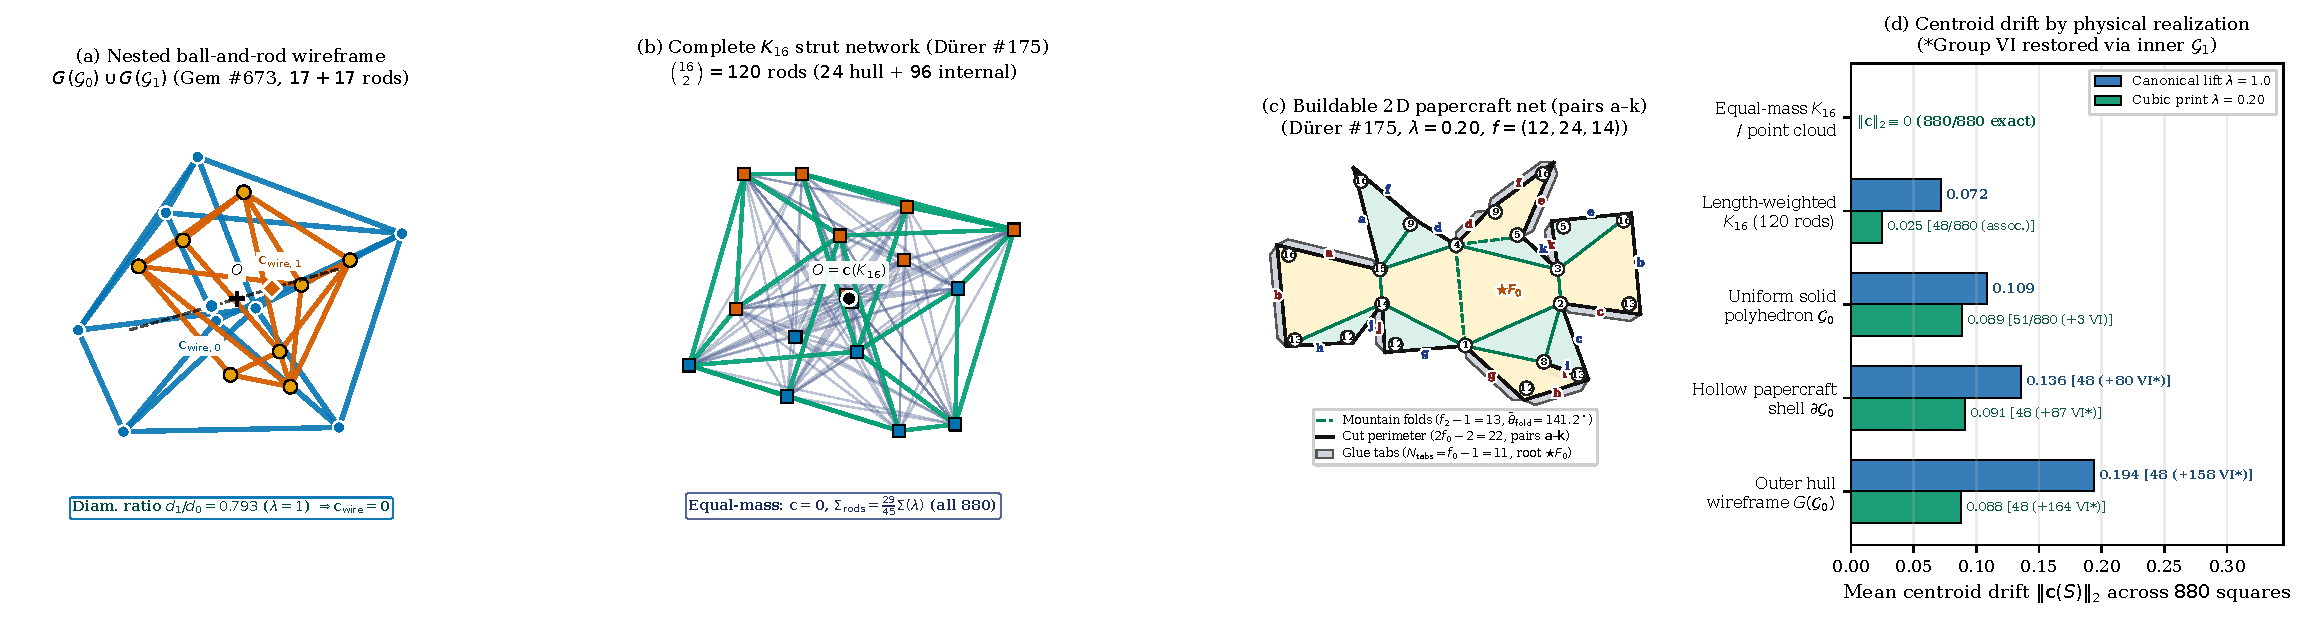
\includegraphics[width=\textwidth]{figures/fig_wireframes_and_nets.pdf}
\caption{Wireframes, complete $K_{16}$ strut networks, and unfolded papercraft cutout nets of Magic Gems \cite{mathewson2025magicgemweb}. (a)~Nested ball-and-rod wireframe $G(\mathcal G_0)\cup G(\mathcal G_1)$ of Gem \#673 ($17$ outer blue rods + $17$ inner orange rods), where tuning the inner-to-outer rod diameter ratio to $d_1/d_0=0.793$ at $\lambda=1$ ($0.493$ at $\lambda=0.20$) restores $\mathbf c_{\mathrm{wire}}=\mathbf 0$. (b)~Fully interconnected complete network $K_{16}$ of D\"urer's Gem \#175 (\texttt{magicGem\_v2.stl}) with all $\binom{16}{2}=120$ rods ($24$ outer hull edges in green + $96$ internal cross-struts in slate) and $16$ node cubes; for equal-mass rods, $\mathbf c(K_{16})=\mathbf 0$ and $\Sigma_{\mathrm{rods}}=\frac{29}{45}\Sigma(\lambda)$ for all $880$ squares (\Cref{thm:complete-network}(1)). (c)~Exact 2D unfolded papercraft cutout net of D\"urer's Gem \#175 ($\lambda=0.20$, $f=(12,24,14)$) rooted at $\bigstar F_0$, with $f_2-1=13$ dashed fold lines (mean dihedral fold angle $\overline{\theta}_{\mathrm{fold}}=141.2^\circ\in[117^\circ,165^\circ]$), $2f_0-2=22$ solid cut perimeter segments, $N_{\mathrm{tabs}}=f_0-1=11$ grey trapezoidal glue tabs paired with their mating cut edges by lowercase labels \texttt{a}--\texttt{k} (\Cref{prop:papercraft-net}(1)), and magic entries $s_{ij}$ at the unfolded vertices. (d)~Comparison of mean centroid drift $\|\mathbf c(S)\|_2$ across all $880$ order-four magic squares for the five physical realizations at $\lambda=1.0$ and $\lambda=0.20$.}
\label{fig:wireframes-nets}
\end{figure}

